\section{Goals and Objectives}
\label{sec:performance-modeling-goals-and-objectives}
\textit{Performance modeling} is the art of studying the behavior of a system in terms of performance metrics in order to maximize the return on tech investments.
To this aim, the \textit{simulation} is the most effective and scalable way to gather system insights and prove performance conjectures without even requiring the existence of the real system.

In this paper, we consider the system architecture in Figure~\ref{fig:system-architecture} and use a simulator to study its behavior with the goal of minimizing the response time.

The system is made of two following layers and accepts classed end-user workloads:

\begin{itemize}
		\item \textbf{Cloudlet:} upfront layer made of one-hop finite resources, having the ability to off-load tasks to the Cloud server, accordingly to an \textit{off-loading policy} based on the occupancy state of the Cloudlet. In particular, the Cloudlet may \textit{forward} incoming tasks to Cloud or \textit{restart} preempted tasks in Cloud with some \textit{overhead}. 
		
		\item \textbf{Cloud:} backfront layer made of a remote Cloud server with virtually unlimited resources.
\end{itemize}

We assume the Cloudlet  providing tasks with higher service rates than the Cloud because, since the former is placed on the network edge, it has lower transmission time and it is less exposed to network latencies.

We propose to evaluate the system behavior with two alternative off-loading policies:

\begin{itemize}
	\item \textbf{Off-Loading Policy 1 (OP1):} the Cloudlet makes no distinction between tasks; it forwards incoming tasks to the Cloud when it has no available resources.
	
	\item \textbf{Off-Loading Policy 2 (OP2):} the Cloudlet gives higher priority to $1^{st}$ class tasks; it accepts only a thresholded occupancy of $2^{nd}$ class tasks, interrupts $2^{nd}$ class tasks to free up resources for $1^{st}$ class tasks and forwards incoming tasks to the Cloud when it has no available resources.
\end{itemize}

We propose to evaluate system stationary and the following performance metrics with a $95\%$ level of confidence:

\begin{itemize}
	\item \textit{System/Cloudlet/Cloud response time} both global and per-class;
	
	\item \textit{System/Cloudlet/Cloud throughput} both global and per-class;
	
	\item \textit{System/Cloudlet/Cloud mean population} both global and per-class;
	
	\item \textit{Cloudlet interruption percentage} of the $2^{nd}$ class tasks;
	
	\item \textit{System response time of interrupted tasks}.
\end{itemize}

\begin{figure}
	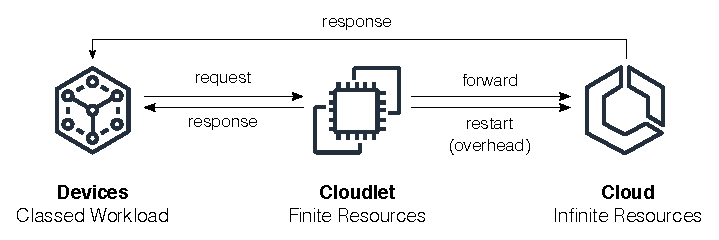
\includegraphics[width=\columnwidth]{fig/architecture}
	\caption{System architecture.}
	\label{fig:system-architecture}
\end{figure}

It is worth studying such a system because it represents the simplest form of a Fog Computing infrastructure, where the end-user workload is  served by Edge compute nodes,  possibly off-loading it to a Cloud provider. The goal of such a study is then to asses the impact of distinct off-loading policies given the trade-off between (i) Edge compute nodes, which are barely exposed to network latencies, but hardly scale and (ii) Cloud compute nodes,  which are virtually infinite, but more exposed to network latencies.